\documentclass{beamer}
\usepackage[english, russian]{babel}
\usepackage{graphicx}
\usepackage{booktabs}
\usepackage{textpos}

\newtheorem*{randomvariable*}{Случайная величина}
\newtheorem{underlying*}{Базовый актив}
\newtheorem{derivative*}{Дериватив}
\newtheorem{futures*}{Фьючерс}
\newtheorem{option*}{Опцион}

\newcommand{\quotes}[1]{``#1''}
\newcommand{\E}{\ensuremath{\mathbb{E}}}
\newcommand{\D}{\ensuremath{\mathbb{D}}}
\renewcommand{\P}{\ensuremath{\mathbb{P}}}
\newcommand{\R}{\ensuremath{\mathbb{R}}}
\newcommand{\Z}{\ensuremath{\mathbb{Z}}}
\newcommand{\Q}{\ensuremath{\mathbb{Q}}}
\newcommand{\LQ}{\ensuremath{\mathcal{L}_{\mathbb{Q}_p}}}
\newcommand{\LZ}{\ensuremath{\mathcal{L}_{\mathbb{Z}_p}}}
\newcommand{\LQn}{\ensuremath{\mathcal{L}^{(n)}_{\mathbb{Q}_p}}}
\newcommand{\LZn}{\ensuremath{\mathcal{L}^{(n)}_{\mathbb{Z}_p}}}
\newcommand{\LQcentralr}{\ensuremath{\mathcal{L}_{\mathbb{Q}_p, n}}}
\newcommand{\Sbf}{\ensuremath{\mathbf{S}}}
\newcommand{\rank}{\ensuremath{\mathrm{rank}}}
\newcommand{\xoo}{\ensuremath{x_{1,1}}}
\newcommand{\xod}{\ensuremath{x_{1,2}}}
\newcommand{\xdo}{\ensuremath{x_{2,1}}}
\newcommand{\xdd}{\ensuremath{x_{2,2}}}
\newcommand{\yoo}{\ensuremath{y_{1,1}}}
\newcommand{\yod}{\ensuremath{y_{1,2}}}
\newcommand{\ydo}{\ensuremath{y_{2,1}}}
\newcommand{\ydd}{\ensuremath{y_{2,2}}}
\newcommand{\Wpn}{\ensuremath{\mathcal{W}^{\mathrm{pol}}_n}}
\newcommand{\Wn}{\ensuremath{\mathcal{W}_n}}
\newcommand{\Wp}{\ensuremath{\mathcal{W}^{\mathrm{pol}}}}
\newcommand{\W}{\ensuremath{\mathcal{W}}}
\newcommand{\Lp}{\ensuremath{\mathcal{L}^{\mathrm{pol}}}}
\newcommand{\SQ}{\ensuremath{S_{\mathbb{Q}_p}}}
\newcommand{\SQn}{\ensuremath{S_{\mathbb{Q}_p, n}}}
\newcommand{\SQr}{\ensuremath{S_{\mathbb{Q}_p, r}}}
\newcommand{\SQo}{\ensuremath{S_{\mathbb{Q}_p, 1}}}
\newcommand{\trace}{\ensuremath{\mathrm{trace}}}

\renewcommand{\width}{\ensuremath{\mathrm{width}}}
\renewcommand{\L}{\ensuremath{\mathcal{L}}}
\renewcommand{\char}{\ensuremath{\mathrm{char}}}

\mode<presentation> {

%\usetheme{default}
%\usetheme{AnnArbor}
%\usetheme{Antibes}
%\usetheme{Bergen}
%\usetheme{Berkeley}
%\usetheme{Berlin}
%\usetheme{Boadilla}
%\usetheme{CambridgeUS}
%\usetheme{Copenhagen}
%\usetheme{Darmstadt}
%\usetheme{Dresden}
%\usetheme{Frankfurt}
%\usetheme{Goettingen}
%\usetheme{Hannover}
%\usetheme{Ilmenau}
%\usetheme{JuanLesPins}
%\usetheme{Luebeck}
%\usetheme{Madrid}
%\usetheme{Malmoe}
%\usetheme{Marburg}
%\usetheme{Montpellier}
%\usetheme{PaloAlto}
%\usetheme{Pittsburgh}
%\usetheme{Rochester}
%\usetheme{Singapore}
\usetheme{Szeged}
%\usetheme{Warsaw}

% As well as themes, the Beamer class has a number of color themes
% for any slide theme. Uncomment each of these in turn to see how it
% changes the colors of your current slide theme.

%\usecolortheme{albatross}
%\usecolortheme{beaver}
%\usecolortheme{beetle}
%\usecolortheme{crane}
\usecolortheme{dolphin}
%\usecolortheme{dove}
%\usecolortheme{fly}
%\usecolortheme{lily}
%\usecolortheme{orchid}
%\usecolortheme{rose}
%\usecolortheme{seagull}
%\usecolortheme{seahorse}
%\usecolortheme{whale}
%\usecolortheme{wolverine}

%\setbeamertemplate{footline} % To remove the footer line in all slides uncomment this line
%\setbeamertemplate{footline}[page number] % To replace the footer line in all slides with a simple slide count uncomment this line

%\setbeamertemplate{navigation symbols}{} % To remove the navigation symbols from the bottom of all slides uncomment this line
}

\newtheorem{remark}{Remark}
\newtheorem{conjecture}{Conjecture}
\newtheorem{theorem*}{Theorem}
\newtheorem{proposition}{Proposition}
\newtheorem{formula}{Formula}




\title[Опционы и Математика]{Опционы и Математика}


\institute[Сбер]
{
    \\

    \centering\Large{Ваня Воробьев}\\
    \vspace{0.5cm}
    \begin{center}
        \small
        \href{https://t.me/v0r0bi0v}{t.me/v0r0bi0v} | \href{tel:+79779996957}{+79779996957} | \href{mailto:ievorobev@edu.hse.ru}{IEVorobyev@sberbank.ru}
    \end{center}
}


\begin{document}
    \begin{frame}
        \titlepage
    \end{frame}

    \begin{frame}{Базовые понятия}
        \begin{randomvariable*}

        \end{randomvariable*}
    \end{frame}

    \begin{frame}{Базовые понятия}
        \begin{randomvariable*}
            \begin{itemize}
                \item Математическое ожидание
                \[
                    \E \hspace{0.1cm}\xi = \int\limits_{-\infty}^{+\infty} xf_{\xi}(x) dx \left( = \sum\limits_{i\in I} x_i \cdot \P(\xi = x_i) \right)
                \]
                \item Дисперсия
                \[
                    \D \hspace{0.1cm}\xi = \E\left[(\xi - \E\hspace{0.1cm} \xi)^2\right]
                \]
            \end{itemize}
        \end{randomvariable*}
    \end{frame}

    \begin{frame}{Какие бывают активы}
        \begin{underlying*}
        \end{underlying*}
    \end{frame}

    \begin{frame}{Какие бывают активы}
        \begin{underlying*}
            \begin{itemize}
                \item Валюта
                \item Товары
                \item Ценные бумаги
                \item Процентная ставка
                \item Что угодно численное
            \end{itemize}
        \end{underlying*}
    \end{frame}

    \begin{frame}{Деривативы}
        \begin{derivative*}[Производный финансовый инструмент]
            Соглашение между двумя сторонами, по которому они принимают на себя обязательство или приобретают право купить или продать базовый актив в установленный срок (или до его наступления) по согласованной цене.
        \end{derivative*}
    \end{frame}

    \begin{frame}{Фьючерсы}
        \begin{futures*}
            Контракт, по которому стороны обязуются купить или продать определенное количество товара по заранее установленной цене в определенную дату в будущем.
        \end{futures*}
    \end{frame}

    \begin{frame}{Опционы}
        \begin{option*}
            Контракт, дающий право (но не обязательство) купить (колл-опцион) или продать (пут-опцион) базовый актив по заранее установленной цене в определенную дату в будущем.
        \end{option*}
    \end{frame}

    \begin{frame}{Расчет стоимости}
        \begin{itemize}
            \item Выплата по деривативу является случайной величиной
            \item Нам нужно найти параметры этой случайной величины
        \end{itemize}
    \end{frame}

    \begin{frame}{Расчет стоимости}
        \begin{itemize}
            \item Выплата по деривативу является случайной величиной
            \item Нам нужно найти параметры этой случайной величины
        \end{itemize}
        \begin{itemize}
            \item Фьючерс на год
            \[
                \mathrm{Price} = \E \left[ p_1 \right]
            \]
            \item Колл опцион на год
            \[
                \mathrm{Price} = \E \left[ \max{(p_1 - p_c), 0} \right]
            \]
        \end{itemize}
    \end{frame}

    \begin{frame}{Расчет стоимости}
        \begin{itemize}
            \item Выплата по деривативу является случайной величиной
            \item Нам нужно найти параметры этой случайной величины
        \end{itemize}
        \begin{itemize}
            \item Фьючерс на год
        \end{itemize}
    \end{frame}

    \begin{frame}{Расчет стоимости}
        \begin{itemize}
            \item Выплата по деривативу является случайной величиной
            \item Нам нужно найти параметры этой случайной величины
        \end{itemize}
        \begin{itemize}
            \item Фьючерс на год
            \[
                \mathrm{Price} = \E \left[ p_1 \right]
            \]
        \end{itemize}
    \end{frame}

    \begin{frame}{Расчет стоимости}
        \begin{itemize}
            \item Выплата по деривативу является случайной величиной
            \item Нам нужно найти параметры этой случайной величины
        \end{itemize}
        \begin{itemize}
            \item Фьючерс на год
            \[
                \mathrm{Price} = \E \left[ p_1 \right]
            \]
            \item Колл опцион на год
        \end{itemize}
    \end{frame}

    \begin{frame}{Расчет стоимости}
        \begin{itemize}
            \item Выплата по деривативу является случайной величиной
            \item Нам нужно найти параметры этой случайной величины
        \end{itemize}
        \begin{itemize}
            \item Фьючерс на год
            \[
                \mathrm{Price} = \E \left[ p_1 \right]
            \]
            \item Колл опцион на год
            \[
                \mathrm{Price} = \E \left[ \max{(p_1 - s, 0)} \right]
            \]
        \end{itemize}
    \end{frame}

    \begin{frame}{Опционы в реальной жизни}
        Предположим мы тренер хоккейной команды и нашей команде хватает ничьи для победы в турнире.
    \end{frame}

    \begin{frame}{Опционы в реальной жизни}
        Предположим мы тренер хоккейной команды и нашей команде хватает ничьи для победы в турнире.
        Проведем аналогию с финансами:
        \begin{itemize}
            \item Разница в счете ~--- базовый актив
            \item При ничьей или победе мы заработаем 1, при поражении 0
        \end{itemize}
    \end{frame}

    \begin{frame}{Опционы в реальной жизни}
        Предположим мы тренер хоккейной команды и нашей команде хватает ничьи для победы в турнире.
        Проведем аналогию с финансами:
        \begin{itemize}
            \item Разница в счете ~--- базовый актив
            \item При ничьей или победе мы заработаем 1, при поражении 0
        \end{itemize}
        Мы проигрываем $-1$ на последних минутах матча.
    \end{frame}

    \begin{frame}{Опционы в реальной жизни}
        Предположим мы тренер хоккейной команды и нашей команде хватает ничьи для победы в турнире.
        Проведем аналогию с финансами:
        \begin{itemize}
            \item Разница в счете ~--- базовый актив
            \item При ничьей или победе мы заработаем 1, при поражении 0
        \end{itemize}
        Мы проигрываем $-1$ на последних минутах матча.

        Меняем вратаря на полевого игрока.
        Проанализируем это решение в нашей терминологии.
    \end{frame}

    \begin{frame}{Как устроен прайсинг деривативов в банке}
        \begin{enumerate}
            \item Математически находим \quotes{наиболее подходящие} свойства случайной величины цены базового актива
            \item Считаем соответсвующее данному деривативу матожидание ~--- либо аналитически, либо численно
        \end{enumerate}
    \end{frame}

    \begin{frame}{Примеры случайных процессов}
        Цены базовых активов моделируются как случайные процессы:
        \begin{itemize}
            \item Винеровский процесс (броуновское движение)
            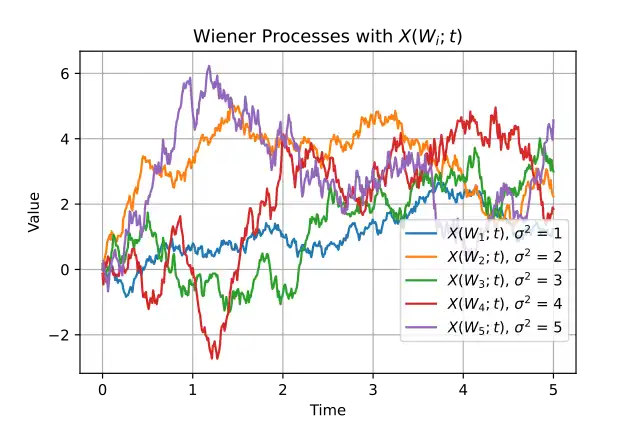
\includegraphics[width=0.7\textwidth]{wiener.png}
        \end{itemize}
    \end{frame}

    \begin{frame}{Примеры случайных процессов}
        Цены базовых активов моделируются как случайные процессы:
        \begin{itemize}
            \item Геометрическое броуновское движение\\
            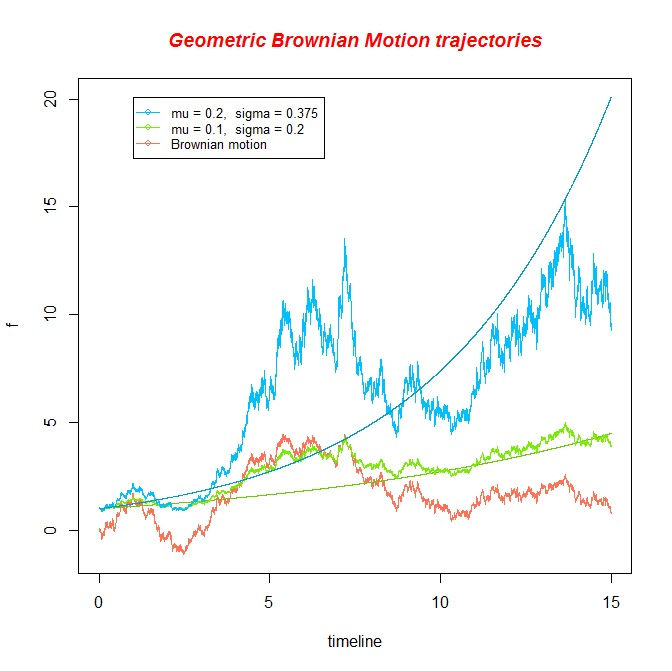
\includegraphics[width=0.5\textwidth]{geometric_brownian_trajectories.jpg}
        \end{itemize}
    \end{frame}

    \begin{frame}{Примеры случайных процессов}
        Цены базовых активов моделируются как случайные процессы:
        \begin{itemize}
            \item Процесс Орнштейна-Уленбека\\
            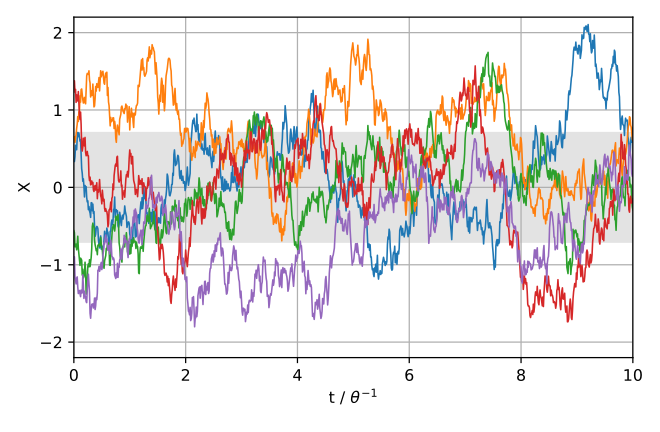
\includegraphics[width=0.7\textwidth]{Ornstein-Uhlenbeck-5traces.svg.png}
        \end{itemize}
    \end{frame}

    \begin{frame}{Исторические цены}
        \begin{itemize}
            \item Евро/Доллар\\
            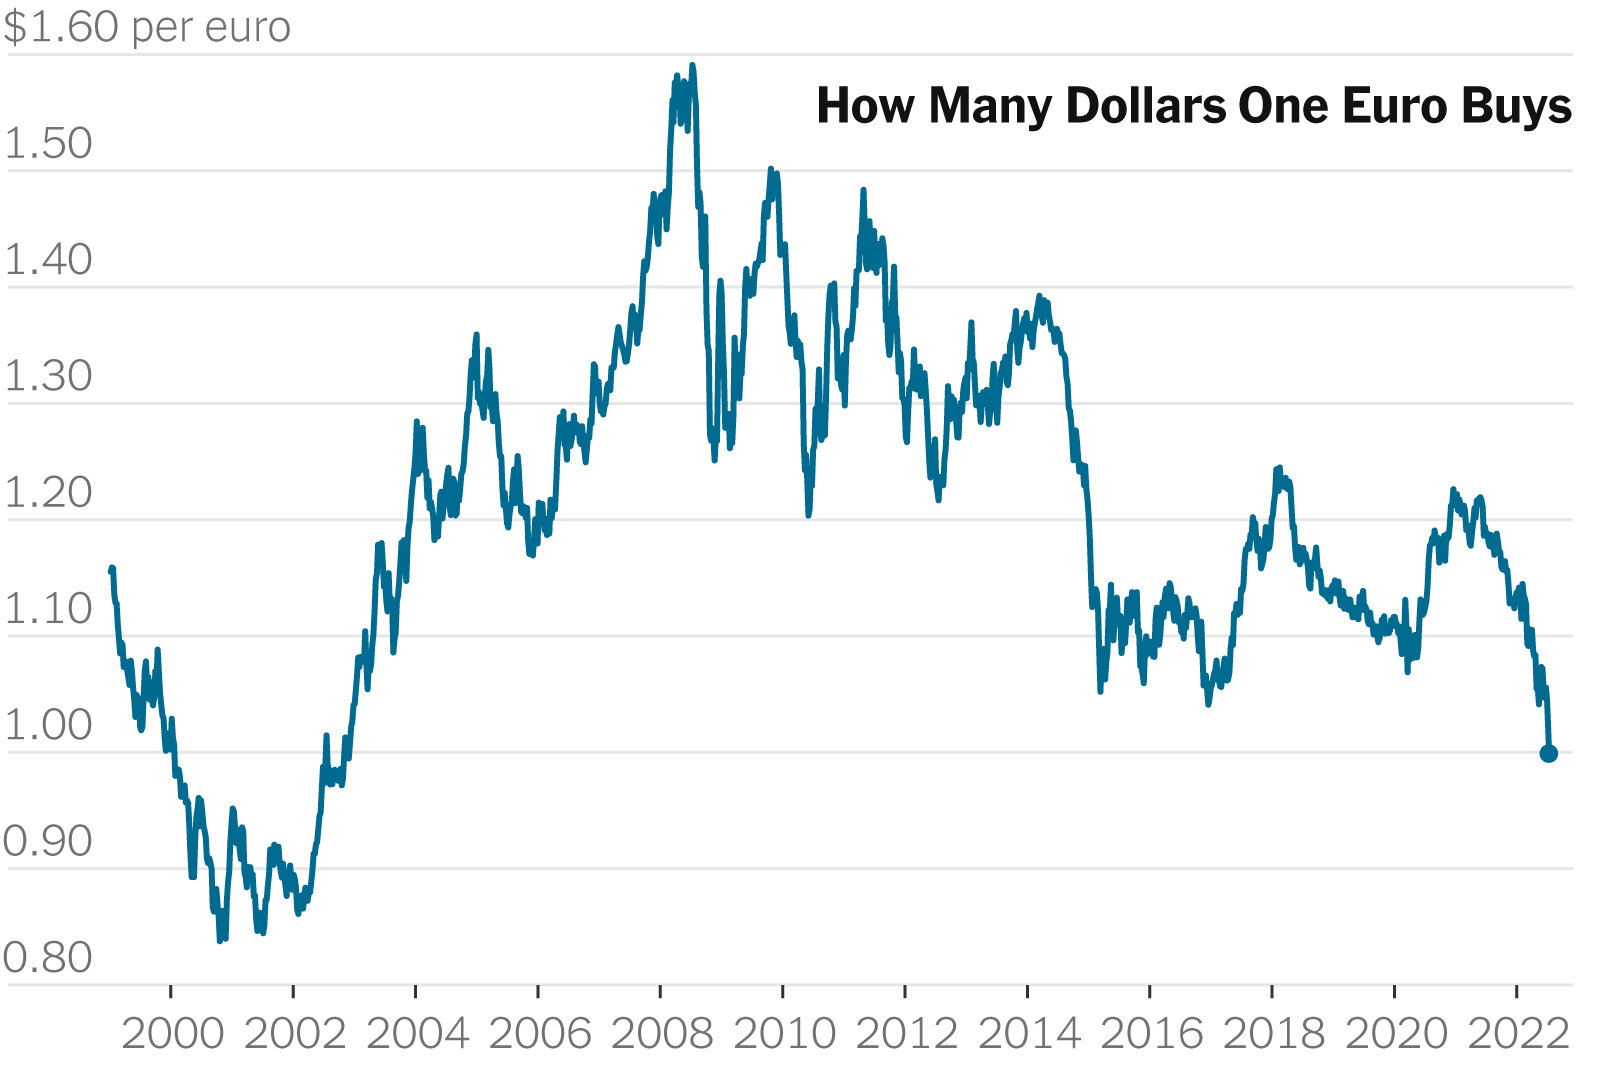
\includegraphics[width=0.7\textwidth]{euro-dollar-parity-alt-promo-superJumbo.jpg}
        \end{itemize}
    \end{frame}

    \begin{frame}{Исторические цены}
        \begin{itemize}
            \item Золото/Доллар\\
            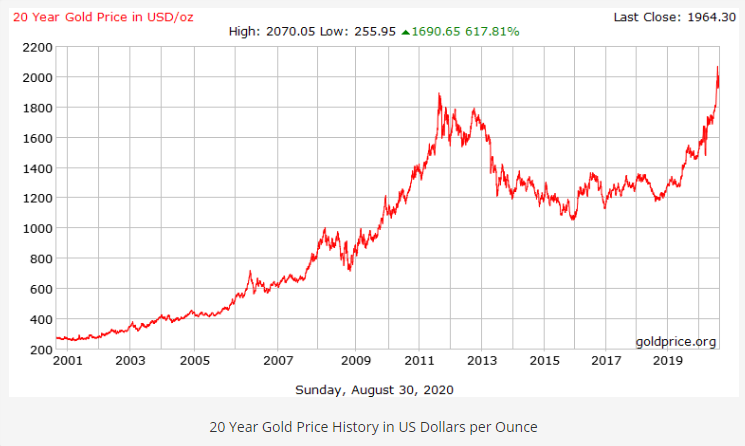
\includegraphics[width=0.7\textwidth]{gold-20y.png}
        \end{itemize}
    \end{frame}

    \begin{frame}{Прайсинг для конкретного случайного процесса}
        Бывает, что хоть случайный процесс и подобран, и матожидание можно написать матожидание, но аналитически его вычислить не получается.

        В таком случае достаточно написать одну строчку кода:
        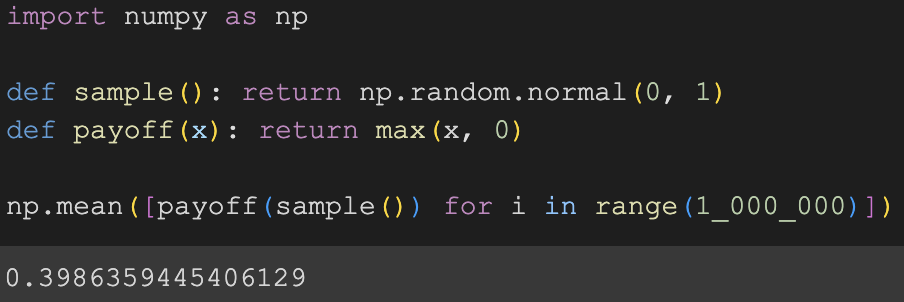
\includegraphics[width=0.7\textwidth]{code.png}

        Однако, конечно бывают и куда более сложные случаи на которые уходят месяцы разработки.

    \end{frame}

%    \begin{frame}{Проблема \quote{простых} процессов}
%        Для простых процессов, таких как GBM можно аналитически посчитать цену европейского колл-опциона.
%        \[
%            \mathrm{Price}\left(\sigma, \mathrm{Strike}\right)
%        \]
%        Можно посмотреть на цены опционов на рынке и выразить $\sigma$ через $\mathrm{Strike}$:
%        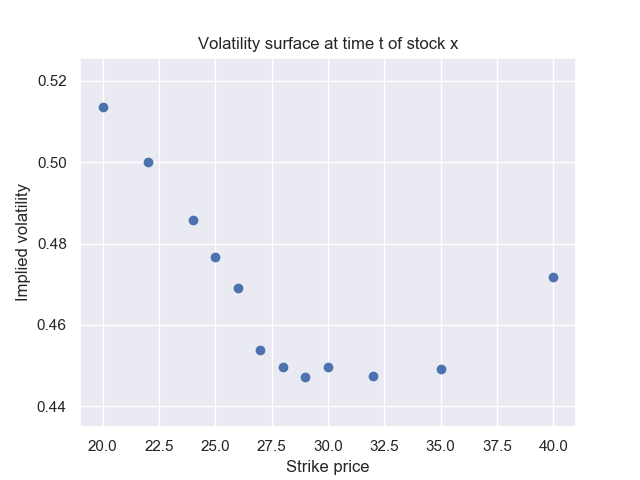
\includegraphics[width=0.3\textwidth]{implied.png}
%    \end{frame}

    \begin{frame}
        \center
        
\includegraphics[width=0.4\textwidth]{me.png}
    \end{frame}
\end{document}
